
\begin{figure*}
  \centering
  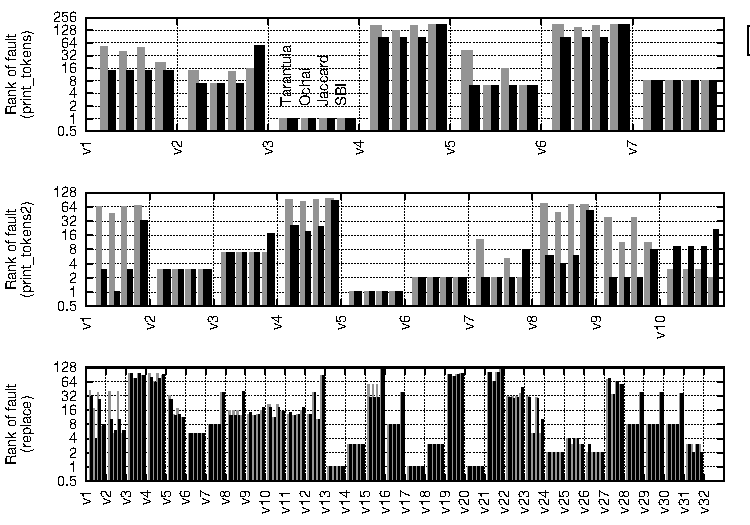
\includegraphics[width=1.8\columnwidth]{siemens1}
  \caption{First Set of SIR Results (Log Scale)}
  \label{fig:allSIR1}
\end{figure*}

\begin{figure*}
  \centering
  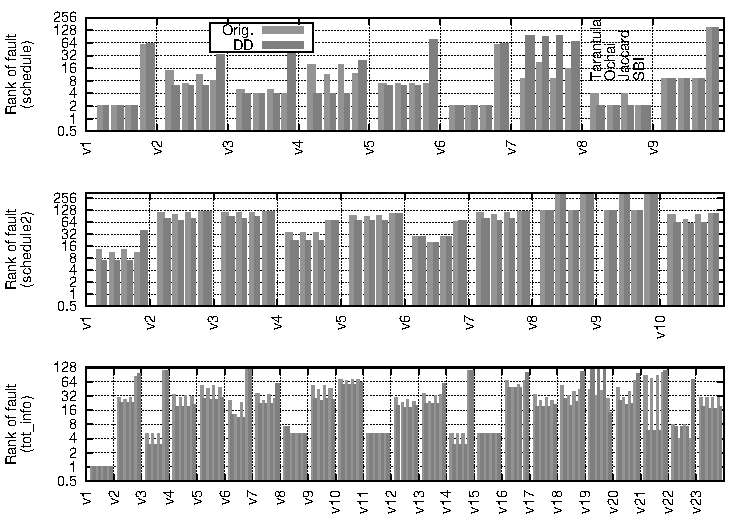
\includegraphics[width=1.8\columnwidth]{siemens2}
  \caption{Second Set of SIR Results (Log Scale)}
  \label{fig:allSIR2}
\end{figure*}


\begin{table}
\begin{center}
\resizebox{\columnwidth}{!}{
\begin{tabular}{|c||c|c|c|c|c|}
\hline
Subject & Avg. & Avg. (DD) & \#Better & \#Same & \#Worse \\
\hline
\hline
{\tt print\_tokens} & 59.7 & 29.7 & 18 & 10 & 0  \\
\hline
{\tt print\_tokens2} & 27.0 & 5.8 & 19 & 17 & 4  \\
\hline
{\tt replace} & 24.5 & 21.8 & 37 & 76 & 11  \\
\hline
{\tt schedule} & 7.7 & 14.3 & 18 & 14 & 4  \\
\hline
{\tt schedule2} & 92.4 & 76.6 & 28 & 12 & 0 \\ 
\hline
{\tt tot\_info} & 29.7 & 17.7 & 75 & 16 & 1 \\
\hline
\hline
{\bf Total} & & & 195 & 145 & 20  \\
\hline
\end{tabular}%
}
\end{center}
%\vspace{-5mm}
\caption{SIR Fault Rank Change Result Frequencies}
\label{tab:avgimproved}
\vspace{-5mm}
\end{table}

Our initial experiments use the Siemens/SIR \cite{doESE05,Siemens}
suite programs studied in many previous papers on fault localization,
in particular the classic evaluation of the Tarantula technique
\cite{Tarantula}.  These subjects provide a large number of faults,
reasonable-sized test suites, and have historically been used to
evaluate localization methods.

Of the seven Siemens programs considered in the empirical evaluation
of Tarantula, only one was unsuitable for delta debugging: TCAS takes
as input a fixed-size vector of integers, and therefore its inputs
cannot be easily decomposed.  For the remainder of the programs, the
input is easily considered as either 1) a sequence of characters or 2)
a sequence of lines, when character-level delta debugging is not
efficient (and so unlikely to be chosen by users in practice), which
was required for the {\tt tot\_info} subject.  In all cases, reduction
took on average less than three seconds per failing test case, an essentially
negligible computational cost.



We evaluated our proposal by 1) first computing the fault ranking for
each version of each subject by the five formulas then 2) performing
the same computation, but using only reduced (by delta-debugging)
versions of the failing tests.  Reduction was performed using Zeller's
delta-debugging scripts, available on the web, and comparing the output
of the original (correct) version of the program and the faulty
version as a pass/fail oracle.

Figures \ref{fig:allSIR1} and \ref{fig:allSIR2} show the
results
%\footnote{Version 32 of {\tt replace} is missing because the fault relies on the library definition of {\tt isalnum}, and is no
%longer present on modern Linux systems, as we determined after
%communicating with Gregg Rothermel and the SIR maintainers.}.  
The
lighter shaded bars show the ranking of the fault, without any
reduction.  The darker bars show the ranking after delta-debugging all
failures.  The graphs are shown in log-scale due to the range of
rankings involved.  In many cases, reducing test cases before
localizing improved the ranking of the fault by a factor of two or
more.  Results for individual subject vary: for {\tt print\_tokens},
the average ranking for faults, over all bugs and all formulas, is
59.5 without reduction, and 36.4 with reduction.  The result is
improved by reduction in 19 cases, remains the same in 15 cases, and
is worse in 1 case.  \comment{These numbers improve to 29.8 average ranking, 18
improvements, and 10 unchanged results.}
Table \ref{tab:avgimproved} shows similar data for all the SIR
subjects.  

Improvement in fault rank after reduction was 1.3 times as common as no change
in rank, and \emph{nearly 10 times as common as worse rank for the
fault.}  In addition to the frequency of improvement of fault rank, it
is also important to examine the degree of improvement (or the
opposite) provided by reduction.  Table \ref{tab:rankchange} shows,
the min, max, and average for changes in rank.  The effect
size when reduction improved rank was usually much larger than the
effect size when it gave worse results.  For {\tt replace}, the
subject with the most instances where reduction made fault ranking
worse, we see that the effect size when reduction was harmful was much
smaller than when reduction was helpful.  Furthermore, when reduction
helped, it often improved the ranking of the fault by more than
\emph{optimally} switching formula  That is, we can ask: if we compare
taking the \emph{worst} formula and applying reduction to improve the
localization, how often is this better than switching to the
\emph{best} localization formula for that subject and fault?
Obviously applying reduction is more practical, since we don't know in
advance which formula will perform best, until we know the correct
result.  By this comparison, it was better to
apply reduction than switch from \emph{worst} to \emph{best} formula
in 36 cases over all SIR subjects;  it was better to switch formula in
only 22 cases.



\begin{table}
\begin{center}
\resizebox{\columnwidth}{!}{%
\begin{tabular}{|c||c|c|c||c|c|c|}
%\hline
\hline
& \multicolumn{3}{|c|}{Better} & \multicolumn{3}{|c|}{Worse} \\
Subject & Min & Max & Avg. & Min & Max & Avg \\
\hline
\hline
{\tt print\_tokens} & 6 & 85 & 44.6 & N/A & N/A & N/A \\
\hline
{\tt print\_tokens2} & 3 & 67 & 45.8 & 6 & 6 & 6.0 \\
\hline
{\tt replace} & 1 & 30 & 9.6 & 1 & 3 & 1.4 \\
\hline
{\tt schedule} & 1 & 15 & 4.8 & 85 & 75 & 81.3 \\
\hline
{\tt schedule2} & 4 & 35 & 22.6 & N/A & N/A & N/A \\
\hline
{\tt tot\_info} & 1 & 81 & 14.7 & 3 & 3 & 3.0 \\
\hline
%\hline
\end{tabular}%
}
\end{center}
\caption{SIR Fault Rank Change Effect Sizes}
\label{tab:rankchange}
\end{table}
